\documentclass{article}
\usepackage{algorithm}
\usepackage{algpseudocode}
\usepackage[utf8]{inputenc}
\usepackage{authblk}
\usepackage{setspace}
\usepackage[margin=1.25in]{geometry}
\usepackage{graphicx}
\usepackage{subcaption}
\usepackage{amsmath}
\usepackage{lineno}
\usepackage{tikz-cd}
\usepackage{hyperref}
\usepackage[style=nejm, citestyle=numeric-comp, sorting=none]{biblatex}

\hypersetup{
    colorlinks=true,
    citecolor=black,
    linkcolor=blue,
    filecolor=magenta,      
    urlcolor=blue,
    pdftitle={Overleaf Example},
    pdfpagemode=FullScreen,
}
\addbibresource{main.bib}

%%%%%% Document Setup %%%%%%

\title{6.4132/16.413 Principles of Autonomy and Decision Making Final Project}
\author[ ]{Toya Takahashi}
\affil[ ]{Massachusetts Institute of Technology}
\affil[ ]{Department of Aeronautics and Astronautics}
\onehalfspacing

%%%%%% Main Text %%%%%%

\begin{document}

\maketitle

\section{Introduction}

Activity planing, motion planning, and trajectory optimization for a robotic arm is challenging. To navigate around an environment, the agent must perform a state space search to plan a sequence of actions and generate a trajectory by using a sample-based planner or modeling the problem as an optimization problem. This project explores 1) defining an activity planning problem with the Planning Domain Definition Language, 2) implementing the Fast-Forward heuristic planner with Enforced Hill Climbing, 3) using RRT with goal-biasing for trajectory generation, and 4) comparing the results with the trajectory generated by constraint optimization. The kitchen simulation environment provides an excellent sandbox for testing and demonstrating the effectiveness of the proposed approach, in addition to learning the benefits and drawbacks of the implemented algorithms.

\begin{figure}[h]
    \centering
    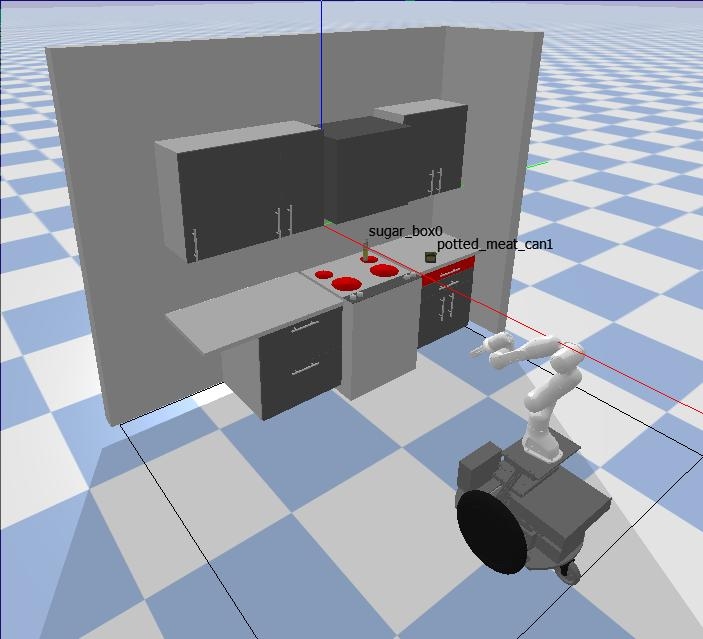
\includegraphics[width=190px]{sim_env.jpg}
    \caption{The kitchen simulation environment}
    \label{fig:sim_env}
\end{figure}

\section{Activity Planning}

\subsection{PDDL Domain and Problem}

The PDDL domain and problem files encode the problem as sets of objects, types, predicates, actions, and goals. There are two main types of objects: the \texttt{box} type, which represents the sugar/spam boxes that are manipulated by the robot arm, and the \texttt{storage} type, which represents the storage spaces in the kitchen. In addition, the \texttt{storage} type is separated into two subtypes: \texttt{static}, which are storage spaces without actions (stovetop burner and countertop), and \texttt{openable}, which are storage spaces that can be opened or closed (drawer, cabinet).

The following assumptions were made when designing the actions and the initial state:
\begin{itemize}
    \item The robot can only grab one box at a time
    \item The robot cannot open drawers or cabinets when gripping an object
    \item Only one box can be placed on each storage space at a time
    \item Drawers and cabinets must be open when placing or picking up a box inside them
    \item Drawers and cabinets must be closed at both the beginning and end of the plan 
\end{itemize}

\begin{figure}[h]
    % https://q.uiver.app/#q=WzAsNSxbMSwwLCJcXHRleHR7b2JqZWN0fSJdLFswLDMsIlxcdGV4dHtzdG9yYWdlfSJdLFsyLDMsIlxcdGV4dHtib3h9Il0sWzAsNiwiXFx0ZXh0e3N0YXRpY30iXSxbMSw2LCJcXHRleHR7b3BlbmFibGV9Il0sWzEsMCwiXFx0ZXh0e2V4dGVuZHN9Il0sWzIsMCwiXFx0ZXh0e2V4dGVuZHN9IiwyXSxbNCwxLCJcXHRleHR7ZXh0ZW5kc30iLDJdLFszLDEsIlxcdGV4dHtleHRlbmRzfSJdXQ==
    \[\begin{tikzcd}
        & {\text{object}} \\
        \\
        \\
        {\text{storage}} && {\text{box}} \\
        \\
        \\
        {\text{static}} & {\text{openable}}
        \arrow["{\text{extends}}", from=4-1, to=1-2]
        \arrow["{\text{extends}}"', from=4-3, to=1-2]
        \arrow["{\text{extends}}"', from=7-2, to=4-1]
        \arrow["{\text{extends}}", from=7-1, to=4-1]
    \end{tikzcd}\]

    \caption{Hierarchical PDDL object types including static/openable storage spaces and boxes}
    \label{fig:types}
\end{figure}

Separating the \texttt{storage} type into subtypes allowed separating the action of placing (and picking up) a box on a storage space into \texttt{place\_static} and \texttt{place\_openable}, which has an extra \texttt{(open ?s)} precondition.

I also did not use any negative preconditions to simplify the implementation of the fast-forward heuristic planner. For actions requiring negative preconditions, I defined a second predicate which is always the negation of the predicate needing to express the negative precondition on (e.g. \texttt{(open ?s - openable)} and \texttt{(closed ?s - openable)}).

\subsection{Fast-Forward Heuristic Planner}

The \texttt{ff\_planner} file contains all functions to solve the activity planning problem. The \texttt{calculate\_hff} function computes the fast-forward heuristic $h_{ff}$ of a given state by counting the number of actions (without delete effects) it takes until the goal condition is a subset of \texttt{state}. At each iteration, \texttt{new\_state} is computed by taking the union of the current state and the add effects of all applicable actions. Because we defined our actions to only have positive preconditions, we can easily determine whether an action is applicable by checking if the precondition is a subset of \texttt{new\_state}.

In this project, I decided to implement Enforced Hill Climbing in the \texttt{solve\_ff} function. While EHC is not guaranteed to find an optimal solution, its greedy nature typically leads to higher efficiency and lower memory usage. \texttt{solve\_ff} initially parses the PDDL files and enumerates all possible actions that can be taken by the agent. Next, it performs a greedy search by adding the first action that leads to a strictly smaller $h_{ff}$ to the plan. If no such action is found, there is a ``plateau" in the graph, and BFS is used to find a sequence of actions that lead to a smaller $h_{ff}$. If BFS fails to find such sequence of actions, then the algorithm determines that the activity planning problem is unsolvable.

Comparing the performance of BFS and FF Heuristic Planner, on the contrary to my expectation, I found that BFS consistently runs faster ($650\mu s$ vs. $950\mu s$). This is because the plan graph is rather simple for this problem. For example, the starting state has $h_{ff}=2$, meaning EHC gets stuck on a ``plateau" for most of the time, resorting to BFS. In this case, calculating $h_{ff}$ leads to computational overhead. For more complex problems requiring many actions to be taken, I expect the FF Heuristic Planner to perform significantly faster than BFS.

\section{Motion Planning}

To view the sample-based motion planner in action, see \href{https://drive.google.com/file/d/1sknWGIKYpLsJexYLzeWbSfdt8TrVTznH/view?usp=sharing}{FF Heuristic Planner and RRT Trajectory Generator} or go to the following url: \url{https://drive.google.com/file/d/1sknWGIKYpLsJexYLzeWbSfdt8TrVTznH/view?usp=drive_link}.

\subsection{Environment Assumptions}

Hard-coded values can be found in \texttt{constants.py} and includes:
\begin{itemize}
    \item The initial 2D poses of the spam and sugar boxes (were not modified significantly from the original positions, simply moved the sugar box closer for the robot arm to reach)
    \item The 3D poses of the spam and sugar boxes after moved by the robot
    \item The 7D goal joint position vectors for the different actions
    \item \texttt{JOINT\_STEP\_SIZE}, \texttt{GOAL\_SAMPLE}, and \texttt{GOAL\_THRESHOLD} (explained in \href{sec:rrt}{Trajectory Generation using RRT})
\end{itemize}

In addition, the following environment assumptions were made:
\begin{itemize}
    \item The sugar/spam box attaches to the end-effector once the ``grab" action finishes
    \item The drawer opens after the ``open drawer" action ends and closes before the ``close drawer" action begins
\end{itemize}

Importantly, the collision detection in my RRT implementation is simplified from traditional methods. Typically, when checking if a newly sampled point can be reached without collisions, RRT calculates whether the line between the new point and its nearest point in the tree intersects with an obstacle. However, in my implementation, I only check whether the new sampled point is inside an obstacle, meaning the robot collides with an object in the kitchen environment. This simplification can be made because the robot bodies are large and the distance between each node in the tree are small, meaning if a new joint configuration does not cause a collision, it is almost guaranteed that all joint configurations between the new point and its closest point are valid.

\begin{figure}[h]
    \centering
    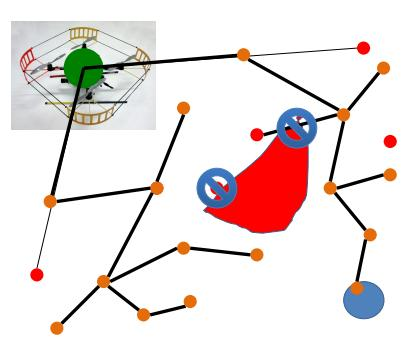
\includegraphics[width=190px]{rrt_collision.jpg}
    \caption{Collision detection in RRT}
    \label{fig:rrt_collision}
\end{figure}


\subsection{Trajectory Generation using RRT}
\label{sec:rrt}

The sample-based motion planning algorithm is written in \texttt{rrt.py}. \texttt{get\_sample\_fn} returns a sampling function that returns a random valid joint configuration $x_\text{rand}$. I also defined a class \texttt{Tree} which keeps track of its \texttt{parent}, \texttt{children}, and \texttt{point} (joint configuration), and has a method \texttt{add\_child} which appends a new \texttt{Tree} to its \texttt{children} and sets the child's \texttt{parent} to itself. 

Class \texttt{TrajectoryGenerator} contains the main motion planning algorithm in the \texttt{solve} method. It also includes four helper functions:
\begin{enumerate}
    \item \texttt{find\_nearest}: returns $x_\text{nearest}$, the node in the tree closest to $x_\text{rand}$ by recursively traversing the tree.
    \item \texttt{steer}: creates a line from $x_\text{nearest}$ to $x_\text{rand}$ limited to length \texttt{JOINT\_STEP\_SIZE}. Returns this new point $x_\text{new}$.
    \item \texttt{obstacle\_free}: returns true if the input joint configuration does not cause the robot to collide with a kitchen object.
    \item \texttt{find\_path}: returns a list of joint configurations from the initial state to the goal state by following the parent pointers.
\end{enumerate}

RRT is then implemented as follows using the helper functions:
\begin{algorithm}
\caption{Rapidly-Exploring Random Tree (RRT)}\label{alg:rrt}
\begin{algorithmic}
\State $\mathtt{tree} \gets \mathtt{Tree()}$
\State $i \gets 1$
\While{\texttt{True}}
    \If{$i\mod\mathtt{GOAL\_SAMPLE}=0$}
        \State $x_\text{rand} \gets x_\text{goal}$
    \Else
        \State $x_\text{rand} \gets \mathtt{sample\_free()}$
    \EndIf
    \State $x_\text{nearest} \gets \mathtt{find\_nearest(tree}, x_\text{rand})$
    \State $x_\text{new} \gets \mathtt{steer}(x_\text{nearest}, x_\text{rand})$
    \If{$\mathtt{obstacle\_free}(x_\text{new})$}
    \State $x_\text{last} \gets \mathtt{Tree}(x_\text{new})$
        \State $x_\text{nearest}\mathtt{.add\_child}(x_\text{last})$
        \If{$\mathtt{dist}(x_\text{new}, x_\text{goal})\le\mathtt{GOAL\_THRESHOLD}$}
            \State \Return{$\mathtt{find\_path}(x_\text{last})$}
        \EndIf 
        \State $i \gets i + 1$
    \EndIf 
\EndWhile
\end{algorithmic}
\end{algorithm}

Instead of getting a random sample every time, the algorithm samples the goal state every \texttt{GOAL\_SAMPLE} cycles to bias the tree. Additionally, we determine whether $x_\text{new}$ is in the goal state by checking if the euclidian distance between $x_\text{new}$ and $x_\text{goal}$ is less than \texttt{GOAL\_THRESHOLD}. 

While the algorithm successfully generates a trajectory as shown in the video, it can be slow depending on the initial and goal state. Constants needed to be tuned to increase the performance of the algorithm.

\subsection{Integration with the Activity Planner}

The \texttt{robot.py} file includes a \texttt{Robot} class with methods for each action in the PDDL domain in addition to methods to move the robot base and arm to the initial state. Dictionary \texttt{function\_map} maps PDDL actions to its corresponding methods, and the \texttt{act} method uses \texttt{function\_map} to perform a task based on a given action.

The overall plan execution is written in \texttt{plan\_executor.py}. The code initially solves the activity planning problem using the FF Heuristic Planner, which returns a list of tasks to execute. \texttt{plan\_executor} simply iterates through this list and calls the \texttt{Robot().act} method for each action to fully execute the plan.

\section{Trajectory Optimization}

To view the trajectory optimization in action, see \href{https://drive.google.com/file/d/1ZB1DUmpl6Mqf19IPNjAWVvW_RhoJtXB6/view?usp=sharing}{Trajectory optimization} or go to the following url: \url{https://drive.google.com/file/d/1ZB1DUmpl6Mqf19IPNjAWVvW_RhoJtXB6/view?usp=sharing}.

\subsection{File organization}

Trajectory optimization is implemented in pydrake using the default IPOPT nonlinear optimization solver, and can be found in \texttt{trajopt.py}. The \texttt{solve} function in the \texttt{TrajectoryOptimizer} class solves the optimization problem defined in \href{sec:opt}{Optimization problem definition} and takes an initial guess of the arm trajectory as an optional argument to seed the solver. Furthermore, the \texttt{Robot} class constructor has an additional \texttt{use\_trajopt} argument which allows the use of \texttt{TrajectoryOptimizer} to generate the arm trajectory. Finally, the trajectories generated from the sample-based motion planner were saved as \texttt{.npy} files in the \texttt{npy} folder. To use these trajectories as inputs to the IPOPT solver, I added a new \texttt{Robot().get\_init\_guess} method which loads a \texttt{.npy} file and linearly interpolates \texttt{PATH\_LENGTH} sample points. The solver generates a trajectory encoded as a $\mathtt{PATH\_LENGTH}\times7$ matrix, so the initial guess must also be of the same size.

\subsection{Optimization problem definition}
\label{sec:opt}

The kinematic trajectory optimization formulation is inspired from the problem used in Professor Russ Tedrake's Robotic Manipulation course \cite{Tedrake}:

\begin{equation*}
\begin{aligned}
    \min_T\quad & T,\\
    \textrm{subject to}\quad & X^{G_{start}}=f_{kin}(q(0)),\\
                             & X^{G_{goal}}=f_{kin}(q(T)),\\
                             & \forall t,\quad |\dot q|\le v_{max},
\end{aligned}
\end{equation*}

Where $f_{kin}$ is the forward kinematics function and $q(t)$ is the joint state of the robot at time $t$. The problem reads as minimizing time $T$ for the arm to move from the start pose $X^{G_{start}}$ to the goal pose $X^{G_{goal}}$ while satisfying velocity constraints. 

There are a few challenges when converting this problem into a pydrake \texttt{MathematicalProgram}. Since pydrake does not allow pybullet functions to be included in its problem formulation, I simplified the problem to input initial and goal joint states rather than poses, and did not encode collision detection. Moreover, pydrake does not allow indexing into a variable using another variable. To avoid this problem, I hard-coded the length of the arm trajectory to be $\mathtt{PATH\_LENGTH}=200$ defined in \texttt{constants.py}. Finally, I approximated the joint velocities as the following: $\dot q\approx \frac{q(t+1)-q(t)}{T/\texttt{PATH\_LENGTH}}\quad\forall t\in\{0,\dots,T-1\}$. Bringing it all together, the new optimization problem is the following:

\begin{equation*}
\begin{aligned}
    \min_T\quad & T,\\
    \textrm{subject to}\quad & q_0=q[0],\\
                             & q_f=q[T],\\
                             & \forall t\in\{0,\dots,T-1\},\quad \frac{q[t+1]-q[t]}{T/\texttt{PATH\_LENGTH}}\le v_{max},\\
                             & \forall t\in\{0,\dots,T-1\},\quad \frac{q[t+1]-q[t]}{T/\texttt{PATH\_LENGTH}}\ge -v_{max}
\end{aligned}
\end{equation*}

where $q_0$ is the initial joint state and $q_f$ is the goal joint state. When running the program, the generated trajectories were smooth but inefficient as the solver found solutions with nonoptimal local minima. While this was alleviated by seeding the solver with initial guesses, it caused the optimized trajectories to be jagged since the given RRT trajectories exhibited a ``shaking" motion. To prevent such trajectories, I added another set of constraints to limit the acceleration of the joints:

\begin{equation*}
\begin{aligned}
    \forall t\in\{0,\dots,T-2\},\quad \frac{(q[t+2]-q[t+1])-(q[t+1]-q[t])}{2T/\texttt{PATH\_LENGTH}}\le a_{max},\\
    \forall t\in\{0,\dots,T-2\},\quad \frac{(q[t+2]-q[t+1])-(q[t+1]-q[t])}{2T/\texttt{PATH\_LENGTH}}\ge -a_{max}
\end{aligned}
\end{equation*}

Compared to the sample-based motion planner, the end result was smoother and more controlled trajectories but slower computation due to the greater number of constraints. Although some actions continued to cause the arm to move inefficiently, this is because the chioces of the goal joints can be improved. Implementing a custom forward kinematics function compatible with pydrake and setting the goal state as $X^{G_{goal}}=f_{kin}(q(T))$ will allow the program to find more optimal trajectories. Finally, to implement collision avoidance, I would encode the kitchen environment in pydrake and prevent the end-effector from colliding with the environment. However, I expect adding these two sets of constraints to significantly slow down computation.

\section{Conclusion}

Using PDDL and the Fast-Forward heuristic planner is an efficient way to encode and solve an activity planning problem. Although the benefits of using the FF heuristic was unclear in this paper, it can improve performance when solving more complicated problems without many heuristic ``plateaus". Both the sample-based motion planner and nonlinear constraint optimization are valid ways to execute the generated plan. However, constraint optimization, with its ability to precisely encode robot dynamics, yielded a smoother and more optimized trajectory compared to the RRT implementation. Using complex algorithms such as RRT* may result in finding an optimal trajectory, but the required computation power may be too high. Similarly, adding more constraints to encode collision avoidance will result in slower computation for the nonlinear optimizer. For both activity and motion planning, it is essential to consider the compromise between runtime and finding a near-optimal solution, and choose the solution that benefits the program the most.

\printbibliography

\end{document}
